\section{Estimation of Model}

Only a single parameter of the model needs to be estimated: $\beta_L$. Again, just as when tuning the parameters driving the wage indirect inference is used. The parameters are tuned the following way. Simulate $N$ individuals. Find the relevant moments of supplied working hours. Find the mean squared distance between the actual supplied working hours and the simulated. Since in this application grid search over the single parameter $\beta_L$ is used, choose the $\beta_L$ corresponding to the lowest mean squared error.

Usually when tuning a dynamic structural model, using simulated methods of moments one would supply the parameters not as part of the state space. The reason for this, is that as the size of the state space expands, it gets exponentially more expensive to solve the model. So the algorithm would go: for a given set of parameters need to be estimated, supply a random initialization. Solve the model for given parameters. Use the solved model to calculate the moments. Use numerical optimization to minimize given optimization problem. However in this application I have chosen to make the parameter part of the state space, since this paper tries to establish that high dimensional dynamic models can be solved using Deep Reinforcement Learning, and therefore not being a limited by the size of the state space.

This paper has implemented the following strategy for tuning the model: I create a grid of 50 points with $\beta_L$ values in the range $[0.2 to 8]$ evenly spaced. I simualte $N=300$ agents for a given value of $\beta_L$ in the grid. Using these 300 hundred agents i can calculate the mean number of supplied hours pr. agent. here it's important to note, that if an agent works 0 hours, they would assume to be out of the workforce and not appear in the statistics, therefore the statistics $\tilde{mu_i}$ calculated for each specific age is:

\begin{equation}
    \tilde{\mu}_i(q) = \E [ H_i \mid H_i > 0, Q_i = q] 
\end{equation}

where $i$ denotes the specific moment which corresponds to a given age. Now using these moments i can calculate the mean squared error between these simulated moments and the actual moments. I can use mean squared error, or rather i let all moments have even weights in the minimization problem, since the economic interpretation is that the number of supplied hours when forty should be not carry more weight in minimization problem than when 30, 50 or any other age. The Objective function can therefore be written as:

\begin{equation}
    MSE_{\beta_L} = \frac{1}{Q_{max} - Q_{min}}\sum_{i \in \{18, \cdots, 60\}} (\tilde{\mu}_i - \mu_i)^2
\end{equation}

where $\mu_i$ is the true average number of supplied ours of women at given age. Again I use \textbf{LIGEF15} supplied by Statistics Denmark to get the numbers of average supplied number of hours. I use the same seed for the simulation, every time the $N$ agents is simulated with a new $\beta_L$ value. I do the estimation for each of the investigated methods in this paper: Value function Iteration, Deep Q-Learning and Double Deep Q-Learning. 

The estimation results yield the following optimal values using VFI: $\beta_L=3.43$, Optimal Values using DQN $\beta_L=3.59$ and optimal value of Double DQN $\beta_L=3.59$. $3.43$ and $3.59$ are neighbouring grid points. I believe it's safe to conclude that these methods yields if not identical, then almost identical results. And I am willing to conclude that using Deep Q-Learning of Double Deep Q-Learning is excellent methods for solving dynamic models.

\begin{table}[ht]
    \centering
    \begin{tabular}{lrrr}
\toprule
{} &  VFI &  DQN & Double DQN \\
\midrule
$\hat{\beta_L}$ & 3.43 & 3.59 & 3.59 \\
\bottomrule
\end{tabular}
    \caption{Estimation of $\beta_L$}
    \label{tab:beta_L_Estimation}
\end{table}

Looking to figure \ref{fig:beta_L_estimation} it can be seen that the estimations follow the same trajectory. The plot shows the log(MSE) for $\beta_L$ values in the range $[0.2, 8]$. Starting with low $\beta_L$ having medium high MSE, falling slightly at around a $\beta_L = 3$ reaching a minimum at about $\beta_L = 3.5$, and after that a sharp raise in MSE is observed. 

\begin{figure}[ht]
\begin{subfigure}{.5\textwidth}
  \centering
  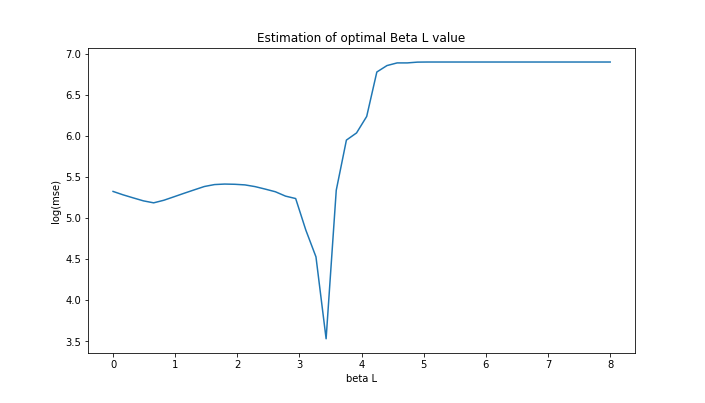
\includegraphics[width=1\linewidth]{figures/dqi_model1_estimation_Beta_L.png}
  \caption{Value Function Iteration Estimation of $\beta_L$}
  \label{fig:dqi_estimation_beta_L}
\end{subfigure}%
\begin{subfigure}{.5\textwidth}
  \centering
  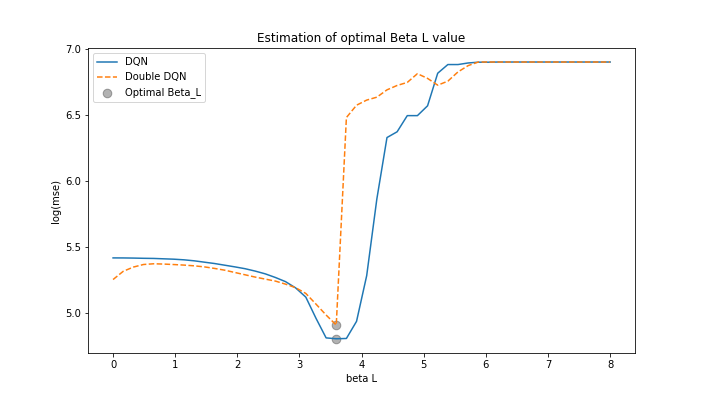
\includegraphics[width=1\linewidth]{figures/dqn_ddqn_model1_estimation_Beta_L.png}
  \caption{DQN and Double DQN estimation of $\beta_L$}
  \label{fig:dqn_ddqn_estimation_beta_L}
\end{subfigure}
    \caption{Estimation of $\beta_L$}
    \label{fig:beta_L_estimation}
\end{figure}

